\documentclass[a4paper]{article}

%% Language and font encodings
\usepackage[english]{babel}
\usepackage[utf8x]{inputenc}
\usepackage[T1]{fontenc}

%% Sets page size and margins
\usepackage[a4paper,top=3cm,bottom=2cm,left=3cm,right=3cm,marginparwidth=1.75cm]{geometry}

%% Useful packages
\usepackage{amsmath}
\usepackage{graphicx}
\usepackage[colorinlistoftodos]{todonotes}
\usepackage[colorlinks=true, allcolors=blue]{hyperref}
\newcommand{\Zp}{\ensuremath{Z^{\prime}}}
\newcommand{\ZpSSM}{\ensuremath{Z^{\prime}_{\mathrm{SSM}}}}
\newcommand{\Z}{\ensuremath{Z}}
\newcommand{\ttbar}{\ensuremath{t\bar{t}}}
\newcommand{\ptSub}[1]{\ensuremath{p_{\text{T} #1}}}
\newcommand{\ptSup}[1]{\ensuremath{p_{\text{T}}^{#1}}}
\newcommand{\pt}{\ensuremath{p_{\text{T}}}}
\newcommand{\ptEl}{\ensuremath{p_{\text{T}}^{e}}}
\newcommand{\ptMu}{\ensuremath{p_{\text{T}}^{\mu{}}}}
\newcommand{\ptZp}{\ensuremath{p_{\text{T}}^{\ensuremath{Z^{\prime}}}}}
\newcommand{\mZp}{\ensuremath{M_{\ensuremath{Z^{\prime}}}}}
\newcommand{\mll}{\ensuremath{M_{\ensuremath{ll}}}}

\def\ifb{\mbox{fb$^{-1}$}}%  Inverse femtobarns.
\def\afb{\mbox{ab$^{-1}$}}%  Inverse femtobarns.

\def\TeV{\ifmmode {\mathrm{\ Te\kern -0.1em V}}\else
                   \textrm{Te\kern -0.1em V}\fi}%
\def\GeV{\ifmmode {\mathrm{\ Ge\kern -0.1em V}}\else
                   \textrm{Ge\kern -0.1em V}\fi}%
\def\MeV{\ifmmode {\mathrm{\ Me\kern -0.1em V}}\else
                   \textrm{Me\kern -0.1em V}\fi}%
\def\keV{\ifmmode {\mathrm{\ ke\kern -0.1em V}}\else
                   \textrm{ke\kern -0.1em V}\fi}%
\def\eV{\ifmmode  {\mathrm{\ e\kern -0.1em V}}\else
                   \textrm{e\kern -0.1em V}\fi}%


\title{FCC Physics: Heavy resonances $\Zp$, RS graviton at $\sqrt{s} = 100 \TeV$}
\author{Clement Helsens Michele Selvaggi, Rachel Smith, Ine Arts}

\begin{document}
\maketitle
\tableofcontents

\begin{abstract}
This document presents a detailed study on the discovery potential of heavy gauge resonance $\Zp$ and 
RS graviton in different decays.
\end{abstract}

\section{Introduction}
This paper 

\section{FCC work flow}
\subsection{Monte-Carlo production}
All the signal Monte-Carlo events have been produced directly with Pythia 

\subsection{Detector parameterizations}
The FCC study group is using the Delphes software package to emulate the response a detector. 
For the FCC one the baseline parameters are:
We also consider two variations around it as well as the CMS configuration.


\subsection{Multi-Variate based selection}
When relevant, in some analyses, a Multi-Variate selection will be performed using the TMVA toolkit.

\subsection{Limit settings}


\section{Physics models}

Models with extended gauge groups often feature additional U(1) symmetries with corresponding heavy spin-1 bosons. These bosons, generally referred to as $\Zp$, would manifest as a narrow resonance through
its  decay,  in  the  dilepton  mass  spectrum.   
Among  these  models  are  those  inspired  by  Grand  Unified Theories, which are 
motivated by gauge unification or a restoration of the left–right symmetry violated
by the weak interaction. Examples are the $\Zp$
bosons of the E6 motivated [1, 2] theories as well as Minimal models [3].  
The Sequential Standard Model (SSM) [2] posits a $\ZpSSM$ boson with couplings to fermions
that are identical to those of the SM $\Z$ boson. This model is a good benchmark as the 
results can be interpreted in the context of other models of new physics, and is useful 
for comparing the sensitivity of different experiments.



\section{Analyses}
\subsection{$\Zp \rightarrow ll$}
\begin{figure}[!htb]\centering
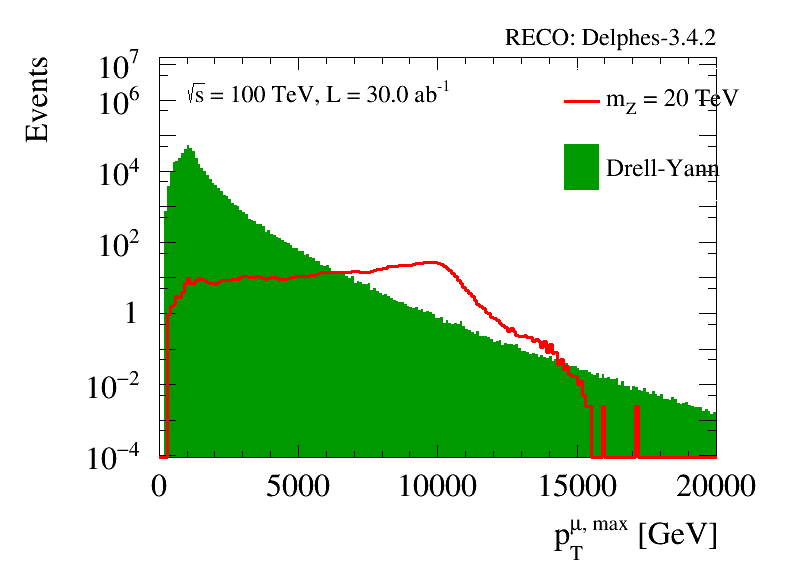
\includegraphics[width=0.495\textwidth]{FCC_ptmu_1_sel0_nostack_log.png}
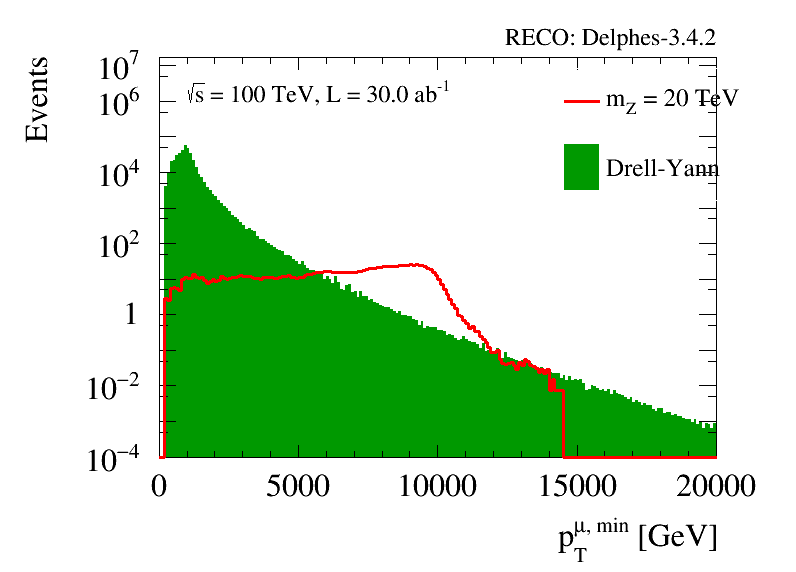
\includegraphics[width=0.495\textwidth]{FCC_ptmu_2_sel0_nostack_log.png}
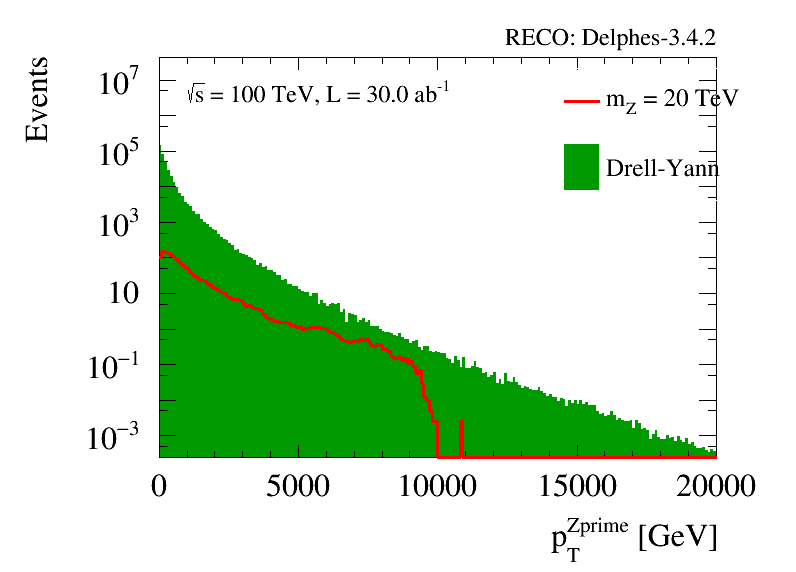
\includegraphics[width=0.495\textwidth]{FCC_ptzp_sel0_nostack_log.png}
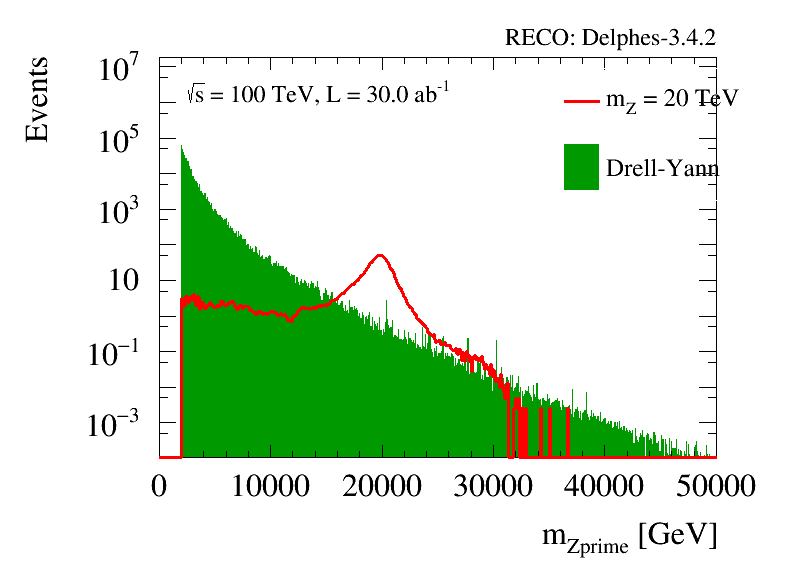
\includegraphics[width=0.495\textwidth]{FCC_mzp_sel0_nostack_log.png}
\caption{Leading (top left) and sub-leading (top right) $\ptMu$, $\ptZp$ (bottom left) and 
di-lepton invariant mass $\mll$ (bottom right) for the FCC 
baseline detector}
\label{fig:zpll_fcc}
\end{figure}


\subsection{$\Zp \rightarrow ll$}
\begin{figure}[!htb]\centering
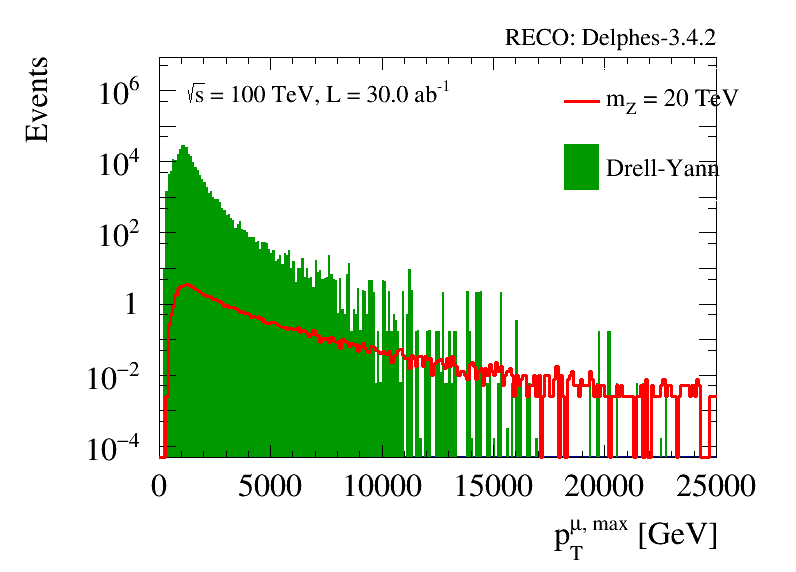
\includegraphics[width=0.495\textwidth]{CMS_ptmu_1_sel0_nostack_log.png}
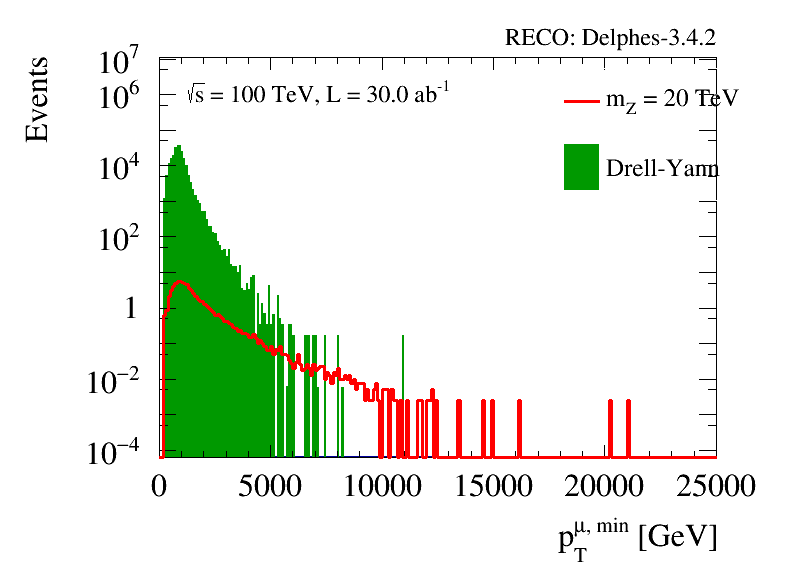
\includegraphics[width=0.495\textwidth]{CMS_ptmu_2_sel0_nostack_log.png}
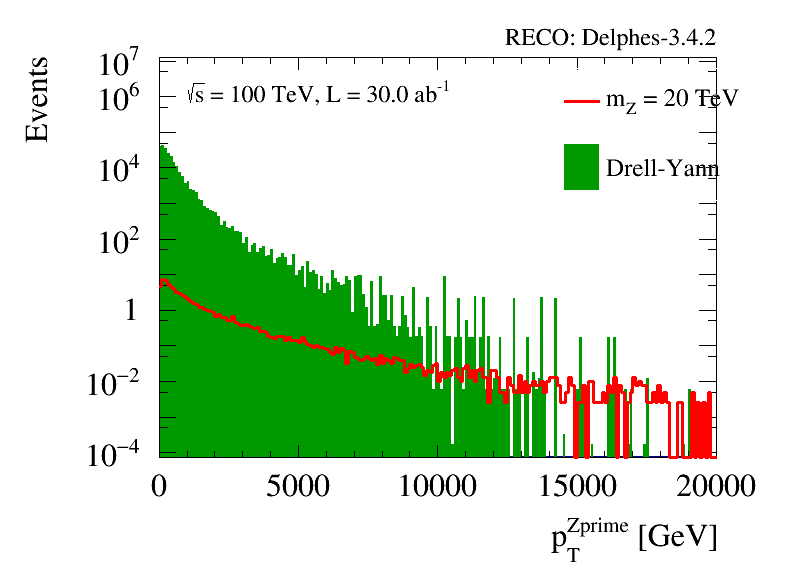
\includegraphics[width=0.495\textwidth]{CMS_ptzp_sel0_nostack_log.png}
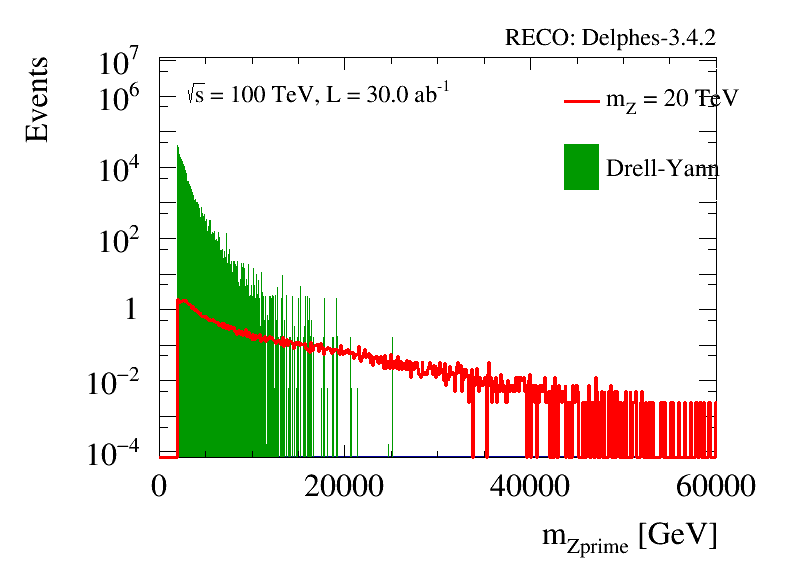
\includegraphics[width=0.495\textwidth]{CMS_mzp_sel0_nostack_log.png}
\caption{Leading (top left) and sub-leading (top right) $\ptMu$, $\ptZp$ (bottom left) and 
di-lepton invariant mass $\mll$ (bottom right) for the CMS  detector}
\label{fig:zpll_cms}
\end{figure}

\begin{figure}[!htb]\centering
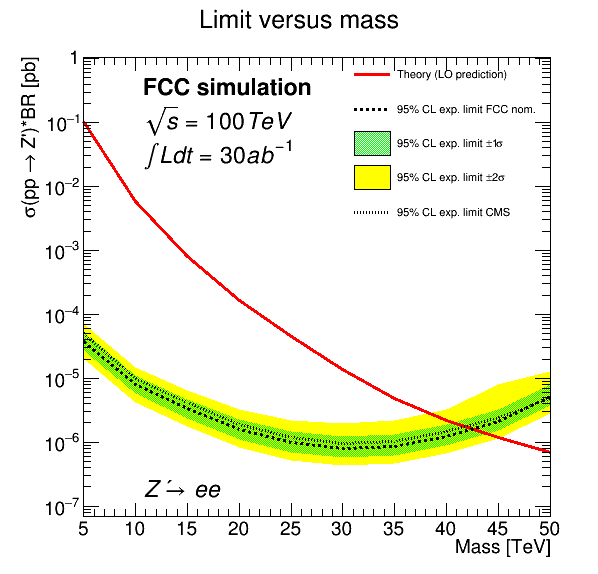
\includegraphics[width=0.495\textwidth]{lim_Zprime_ee_fcc_cms.png}
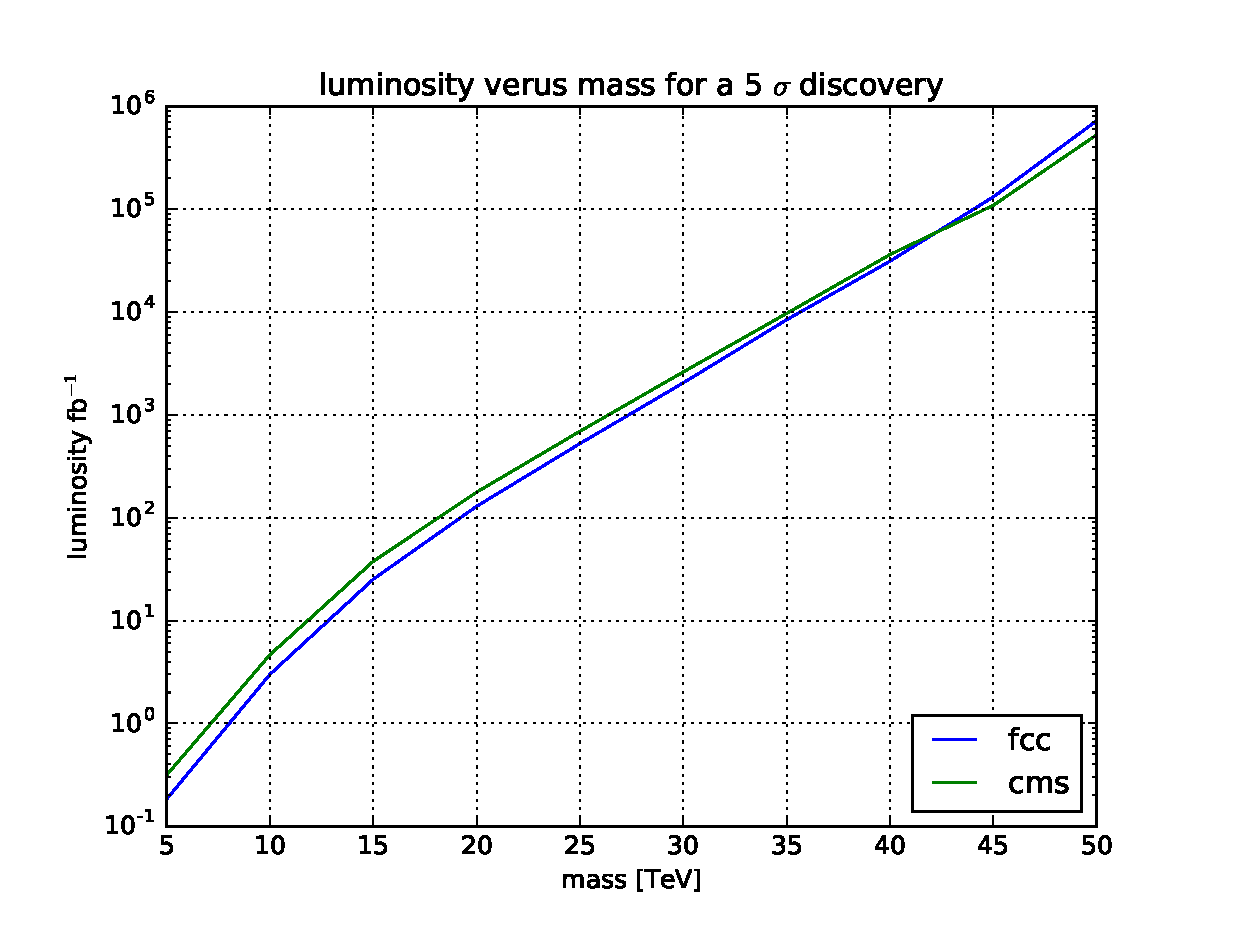
\includegraphics[width=0.495\textwidth]{DiscoveryPotential_ee.eps}
\caption{Limit versus mass (left) and luminosity for a $5\sigma$ discovery (right) for the
 di-electron channel.}
\label{fig:zpee_lim}
\end{figure}

\begin{figure}[!htb]\centering
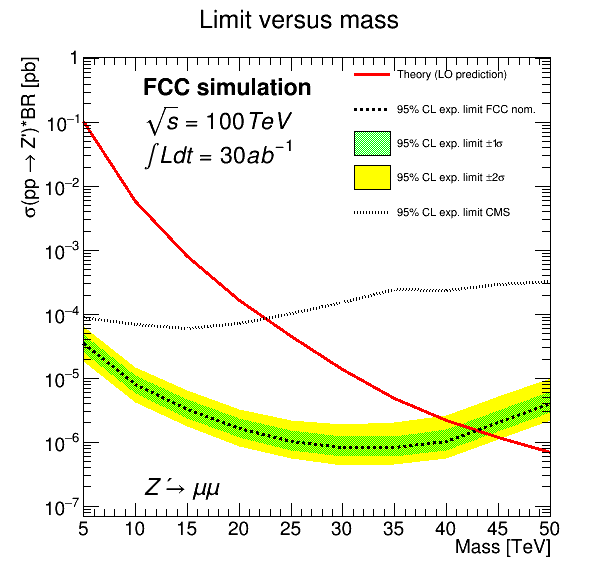
\includegraphics[width=0.495\textwidth]{lim_Zprime_mumu_fcc_cms.png}
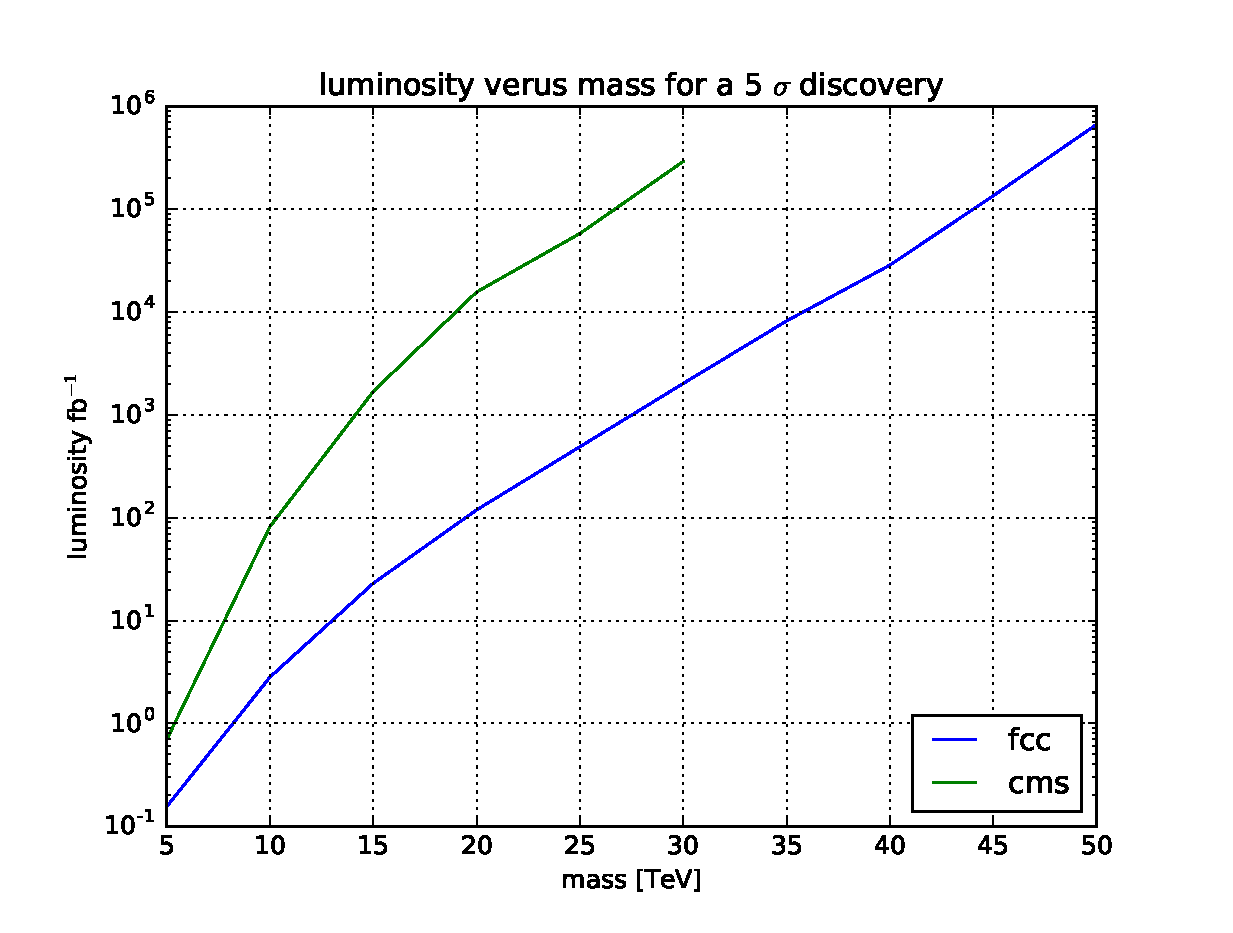
\includegraphics[width=0.495\textwidth]{DiscoveryPotential_mumu.eps}
\caption{Limit versus mass (left) and luminosity for a $5\sigma$ discovery (right) for the
 di-muon channel.}
\label{fig:zpmumu_lim}
\end{figure}

\begin{figure}[!htb]\centering
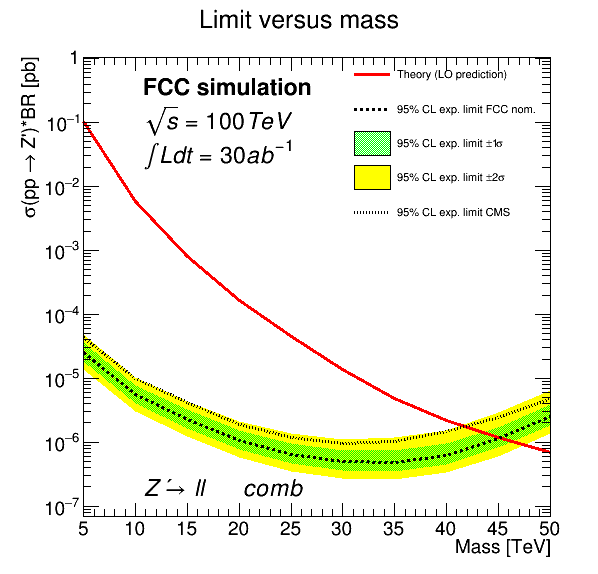
\includegraphics[width=0.495\textwidth]{lim_Zprime_ll_fcc_cms.png}
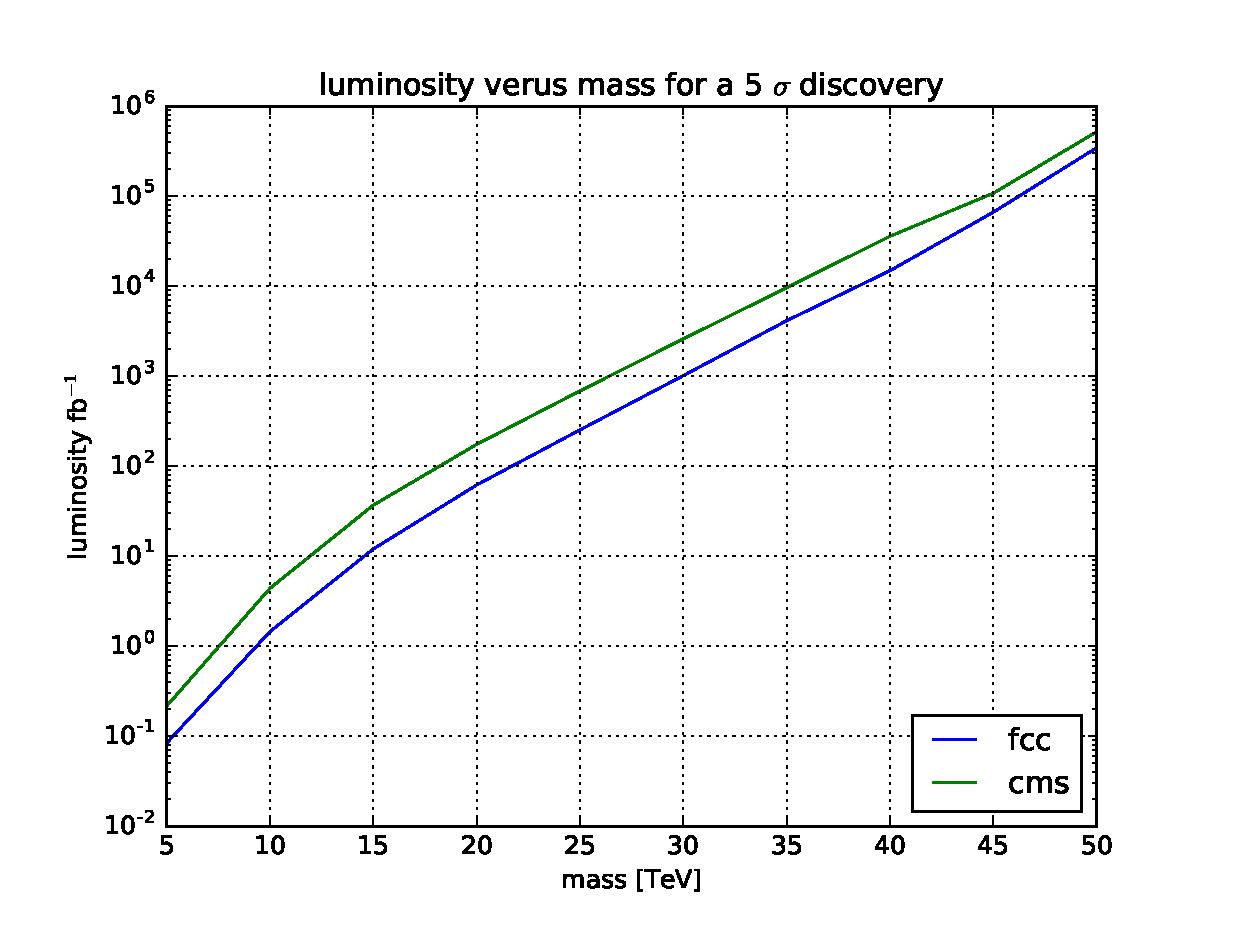
\includegraphics[width=0.495\textwidth]{DiscoveryPotential_ll.eps}
\caption{Limit versus mass (left) and luminosity for a $5\sigma$ discovery (right) for the
 di-lepton channel combined.}
\label{fig:zpll_lim}
\end{figure}

\subsection{$\Zp \rightarrow \ttbar$}
\subsection{$G \rightarrow WW$}
\section{Conclusion}
This note presents preliminary studies of a search for $\Zp$ 
bosons decaying into two electrons or muons in the FCC context. The expected number 
of signal and background events have been estimated from simulated truth level information 
after applying smearing functions to mimic the FCC detector response.
Using a cut-based analysis and assuming simplistic systematic uncertainties, $\ZpSSM$
masses below 40 $\TeV$ can be excluded at 95$\%$ C.L. 
using 30 $\afb{}$ of data. 

\bibliographystyle{plain}
\bibliography{bibliography.bib}
\end{document}